% Optional normalization comparison. Include from the main deck; do not compile alone.
\ifdefined\poreaccessappendixstarted\else\appendix\def\poreaccessappendixstarted{1}\fi
\section[Normalization appendix]{Optional appendix: diffusivity normalization}
\begin{frame}{}
\vfill
{\large\color{tumgray}Optional comparison}\par\vspace{0.4cm}
{\LARGE\color{tumblue}\textbf{The diffusivity-normalized descriptor}}\par\vspace{0.5cm}
{\large Definition, length convention and comparison with direct conductance}
\vfill
\end{frame}
\begin{frame}{Dimensional normalization is an optional descriptor choice}
\begin{columns}[T,onlytextwidth]
\column{0.48\textwidth}\small
\hi{Conductance and diffusivity units}
\[G_{\rm access}=\dot n/\Delta c\quad [\mathrm{m^3/s}]\]
\[D_{\rm access}=G_{\rm access}H/A_{\rm tube}\quad [\mathrm{m^2/s}]\]
For a uniform sample, $G=DA/L$. Multiplication by $L/A$ removes that sample's area-to-length dependence.
\column{0.48\textwidth}\small
\hi{Length is a modelling convention}
\begin{itemize}
\item These comparisons use the full bed height $H$.
\item The steady conductance ends at an interior plane, not the bed top.
\item Dimensional analysis does not select $H$ or establish $D_{\rm access}=D_{\rm eff}$.
\end{itemize}
\end{columns}
\medskip
\result{The main deck uses $G_{\rm access}$ directly; normalization offers no demonstrated advantage in this ensemble.}
\end{frame}
\begin{frame}{Alternative: power law using the normalized descriptor}
  \begin{columns}[c,onlytextwidth]
    \column{0.65\textwidth}
    \centering
    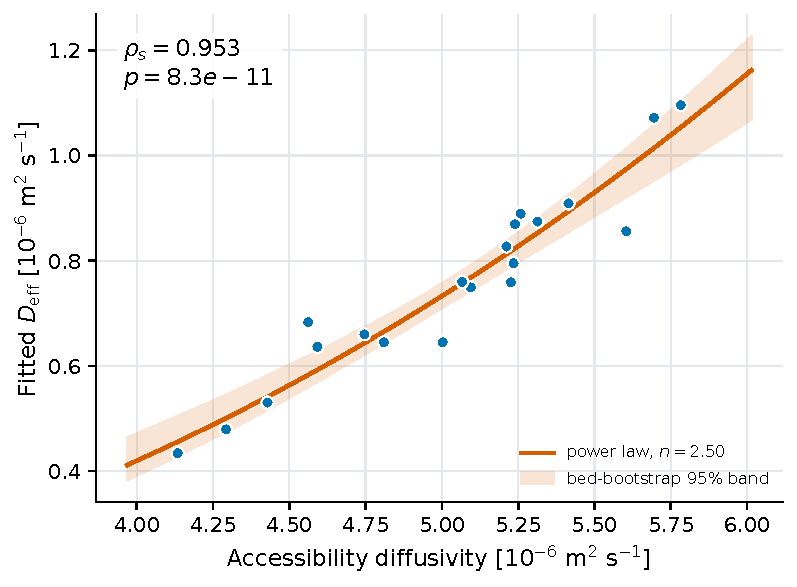
\includegraphics[width=\linewidth,height=0.69\textheight,keepaspectratio]{figures/fig_closure_power_law.pdf}
    \column{0.32\textwidth}
    \small
    \hi{Selected closure}
\[
 \frac{D_{\rm eff}}{D_m}=C\left(\frac{D_{\rm access}}{D_m}\right)^n.
\]
\[
 D_{\rm access}=\frac{G_{\rm access}H}{A_{\rm tube}}.
\]
\medskip
The shaded band shows bootstrap uncertainty in the fitted relationship.
  \end{columns}
  \vspace{0.12cm}
  {\small\result{The fitted exponent is $n\approx2.50$ for this ensemble.}}
\end{frame}

\begin{frame}{Normalized descriptor and raw-conductance linear comparison}
  \begin{columns}[c,onlytextwidth]
    \column{0.62\textwidth}
    \centering
    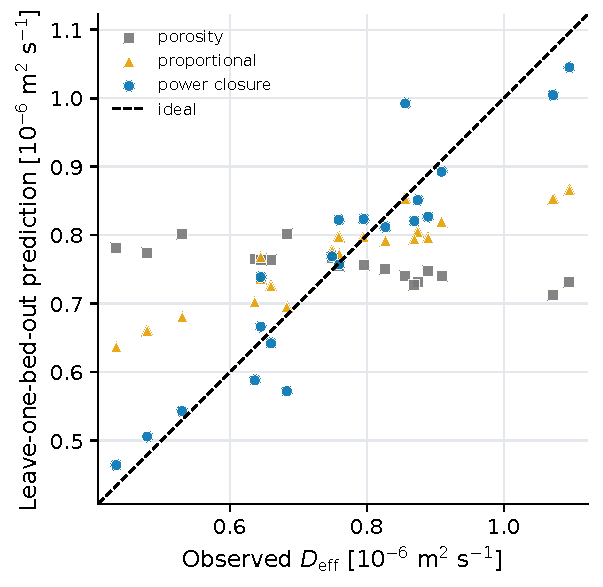
\includegraphics[width=\linewidth,height=0.69\textheight,keepaspectratio]{figures/fig_closure_held_out.pdf}
    \column{0.35\textwidth}\small
    \hi{Forms and held-out $R^2$}
    \begin{tabular}{lr}\toprule
    Predictor / form & $R^2$\\\midrule
    $a_GG_{\rm access}+b_G$ & 0.898\\
    $CD_m(D_{\rm access}/D_m)^n$ & 0.890\\
    $a_DD_{\rm access}+b_D$ & 0.881\\
    $\alpha D_{\rm access}$ & 0.555\\
    $a_0+a_1\varepsilon_b$ & $-0.234$\\\bottomrule
    \end{tabular}
    \medskip\par
    Each expression predicts $D_{\rm eff}$.
    Fit on nineteen beds and predict the omitted bed.
  \end{columns}
  \vspace{0.12cm}
  {\small\result{Power-law and linear-with-intercept scores are close; the power law is not the outright winner.}}
\end{frame}

\begin{frame}{Depth sensitivity of the normalized alternatives}
  \begin{columns}[c,onlytextwidth]
    \column{0.63\textwidth}\centering
    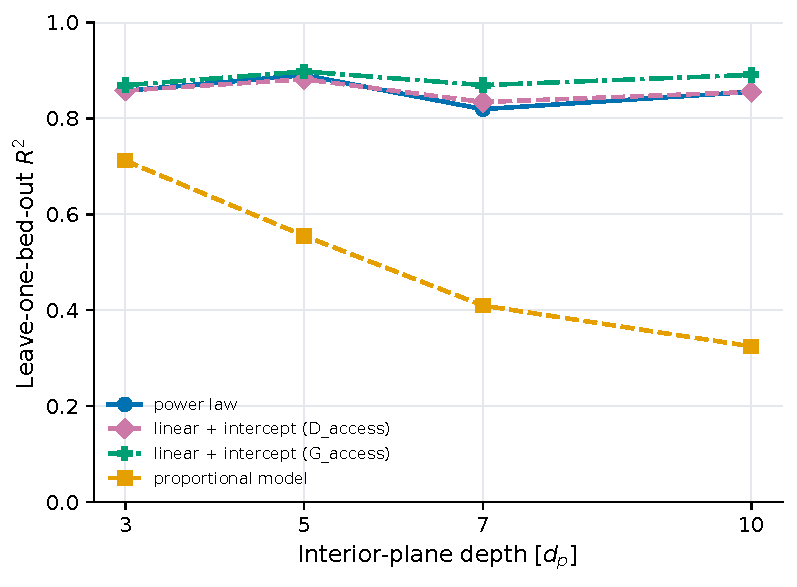
\includegraphics[width=\linewidth,height=0.69\textheight,keepaspectratio]{figures/fig_depth_prediction.pdf}
    \column{0.34\textwidth}\small
    \hi{Four transport models}\par\medskip
    Power law\par
    $D_{\rm eff}=CD_m(D_{\rm access}/D_m)^n$\par\smallskip
    Linear in $D_{\rm access}$ + intercept\par
    $D_{\rm eff}=a_DD_{\rm access}+b_D$\par\smallskip
    Linear in $G_{\rm access}$ + intercept\par
    $D_{\rm eff}=a_GG_{\rm access}+b_G$\par\smallskip
    Proportional\par
    $D_{\rm eff}=\alpha D_{\rm access}$\par\medskip
    Refit on nineteen beds at each depth; predict the omitted bed.
  \end{columns}
  \vspace{0.12cm}
  {\small\result{Power-law $R^2=0.819$--$0.890$ across depths; no consistent advantage over the linear models.}}
\end{frame}
